\documentclass[11pt, oneside]{article}   	% use "amsart" instead of "article" for AMSLaTeX format
\usepackage{geometry}                		% See geometry.pdf to learn the layout options. There are lots.
\geometry{letterpaper}                   		% ... or a4paper or a5paper or ... 
%\geometry{landscape}                		% Activate for for rotated page geometry
%\usepackage[parfill]{parskip}    		% Activate to begin paragraphs with an empty line rather than an indent
\usepackage{graphicx}				% Use pdf, png, jpg, or eps� with pdflatex; use eps in DVI mode
\usepackage{amsmath}								% TeX will automatically convert eps --> pdf in pdflatex		
\usepackage{amssymb}
\setlength{\parindent}{0cm}

\title{Topics in Discrete Math}
\author{Yulong Yang}
%\date{}							% Activate to display a given date or no date

\begin{document}
\maketitle
%\section{}
%\subsection{}

\section{Logic type}

\subsection{propositional}

A proposition is a declarative sentence that is either true or false, but not both. It declares a fact.

Example:

\begin{itemize}
\item ``Washington, D.C., is the capital of the U.S.A.
\item 1 + 1 = 3
\end{itemize}

\subsection{predicate}

Predicate logic usually contains a \textit{variable} and a \textit{predicate}. Without assigning values to the variable, the logic is neither true or false. For example ``$x$ is greater than 3", variable is $x$, and ``is greater than 3" is the predicate, refers to a property the variable could have. If we assign the predicate to be $P(x)$, then it becomes \textit{propositional function} $P$ at $x$. $P(x)$ is a proposition once we assign value to $x$.

Example:
\begin{itemize}
\item $x$ is greater than 3
\item Computer $x$ is under attack
\end{itemize}

\subsection{quantification}

The extent to which a predicate is true over a range of elements (for the variable). Mostly use words like ``all", ``some", etc.

\subsection{logic examples}

\begin{itemize}
\item $p \rightarrow q$: is the proposition ``if p then q", which is false iif $p$ is true and $q$ is false [\textit{propositional}]
\item $\forall xP(x)$: true iif for $P(x)$ is true for every $x$ in the domain [\textit{predicate}]
\end{itemize}

\section{Set}

A set $S$ is closed under addition if for any $x,y \in S$ we have also $x+y \in S$. Also, it is closed under multiplication if $x \times y \in S$.

\section{Regular expression}

\begin{itemize}
\item $\phi$ indicates empty language. In the finite machine, it means start state could be accepted immediately
\item $X+Y$ should expect either $X$ or $Y$, but not both
\item $XY$ should expect first $X$ then $Y$
\item $X^*$ should expect 0 or more $X$s
\item $X^+$ should expect 1 or more $X$s
\end{itemize}

\section{Order notation}

\begin{itemize}
\item $f(n) \in O(g(x))$: there are constants $C$ and $k$ such that $|f(x)| \leq C|g(x)|$ for any $x > k$
\item $f(n) \in \Omega(g(x))$: replace $\leq$ with $\geq$
\item $f(n) \in \Theta(g(x))$: both above two stand correct
\end{itemize}

Master theorem in Figure~\ref{fig:mt}. Use it to solve any recurrence problems.

\begin{figure}[htpb]
\begin{center}
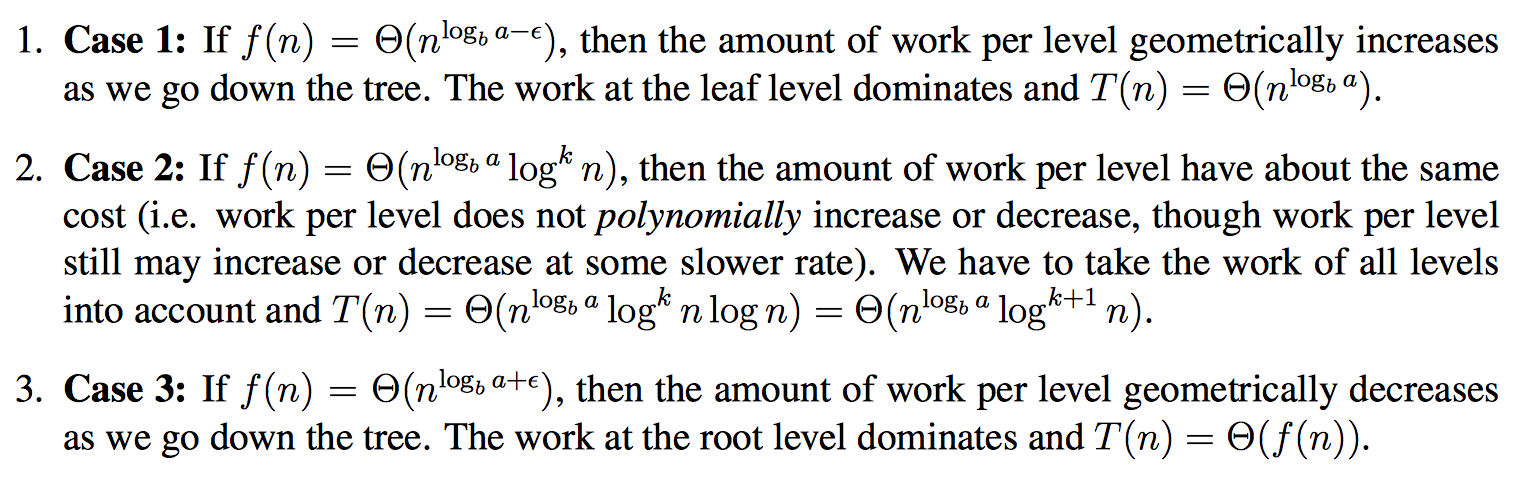
\includegraphics[width=\textwidth]{master.png}
\caption{Master Therorem}
\label{fig:mt}
\end{center}
\end{figure}


\section{Graph}

Planar graph,
\begin{itemize}
\item a graph that could be drawn without any edges crossing (planar representation)
\item Euler's formula: given $e$ edges, $v$ vertices and $r$ regions in a planar representation, we have $r = e - v + 2$
\end{itemize}

\end{document}  